\documentclass[10pt,a4paper]{article}
\usepackage[margin=1.8cm]{geometry}
\usepackage[T1]{fontenc}
\usepackage{lmodern}
\usepackage{graphicx,booktabs,tabularx,amsmath,xcolor,hyperref,float,caption}
\hypersetup{colorlinks=true,linkcolor=blue!50!black,urlcolor=blue!50!black}
\captionsetup{font=small,skip=3pt}
\setlength{\parskip}{3pt}\setlength{\parindent}{0pt}
\setlength{\textfloatsep}{8pt}\setlength{\intextsep}{6pt}
\usepackage{titlesec}
\titlespacing*{\section}{0pt}{8pt}{3pt}
\titlespacing*{\subsection}{0pt}{6pt}{2pt}
\usepackage{enumitem}
\usepackage{multicol}
\newcounter{tech}\renewcommand{\thetech}{A\arabic{tech}}
\newcommand{\tech}[2]{\refstepcounter{tech}\label{app:#2}\paragraph{\thetech\ #1.}}
\newcommand{\app}[1]{(App.~\ref{app:#1})}\setlength{\columnsep}{14pt}
\setlist{nosep,leftmargin=*}
\titlespacing*{\paragraph}{0pt}{4pt}{6pt}

\title{\textbf{Opinion Network Formation from a Class Survey}\\ \large Dynamical Processes in Complex Networks, Assignment 1}
\date{}

\begin{document}
\maketitle
\vspace{-1.8cm}

\section{Team Name}
ConsistentProcess. Members: Vedant Pahariya (2023112012), Siddhant Gudwani (2024102042), Krishna Goel (2023112009).

\section{GitHub Link to Code}
\url{https://github.com/SiddGud/DPCN-opinion-network}. Running \texttt{python src/run\_all.py} rebuilds every figure and number in this report (seed 42). \texttt{data\_prep.py} cleans and encodes the survey, \texttt{network.py} builds the networks, \texttt{analysis.py} computes metrics and null models, \texttt{plots.py} draws figures. Every technique is explained in plain words in the Appendix; references such as (App.~A3) point to the relevant entry.

\section{Dataset Documentation}
The survey has 96 responses to 60 Likert statements, 15 per theme: Technology (T01 to T15), Education (E), Society and Ethics (S) and Environment (V). Each answer is Strongly Disagree, Disagree, Neutral, Agree, Strongly Agree or No Comments.

\subsection{Encoding}
Strongly Disagree $=-2$ up to Strongly Agree $=+2$, so the sign gives the direction of an opinion and the size its strength \app{likert}. ``No Comments'' (37 answers) is treated as missing: a student who declines to answer has not given a neutral opinion.

\subsection{Cleaning}
We removed 5 empty responses and 4 that answered fewer than 30 of 60 statements (they answered only one section, so their similarity to others would rest on too few answers). 87 students remain. The 505 blank cells are treated as missing and never filled in; when comparing two students we use only statements both answered. Blanks grow along the survey (about 5 per statement in Technology, 11 in Environment), which suggests fatigue.

\subsection{Careless answers}
Eight students have a streak of 20 or more identical answers (longest: 42 ``Strongly Agree''). A streak alone does not prove carelessness here, because most statements are easy to agree with; the 42-streak student still disagreed with compulsory attendance and with exams measuring knowledge. We flagged a student only if two of four signs applied (streak $\ge 20$; over 40\% Neutral or No Comments; agreeing with both E01 ``projects beat exams'' and E02 ``exams measure knowledge''; answer SD below 0.5). Three students were flagged and kept; removing them barely changes the results (Section 5.5).

\subsection{What the answers look like}
79\% of the 5{,}255 answers are Agree or Strongly Agree (Fig.~\ref{fig:dist}). Some statements are near unanimous (E15 ``continuous learning is essential'', mean $+1.71$). Only a few divide the class: E04 (online learning), E02 (exams), T08 (AI diagnosis), T09 (autonomous vehicles) and E03 (compulsory attendance, rejected by 70\%). This shapes the pipeline: two students who both agree with 50 easy statements would look similar even if they disagree on everything that matters.

\begin{figure}[H]\centering
\begin{minipage}{0.44\linewidth}\centering
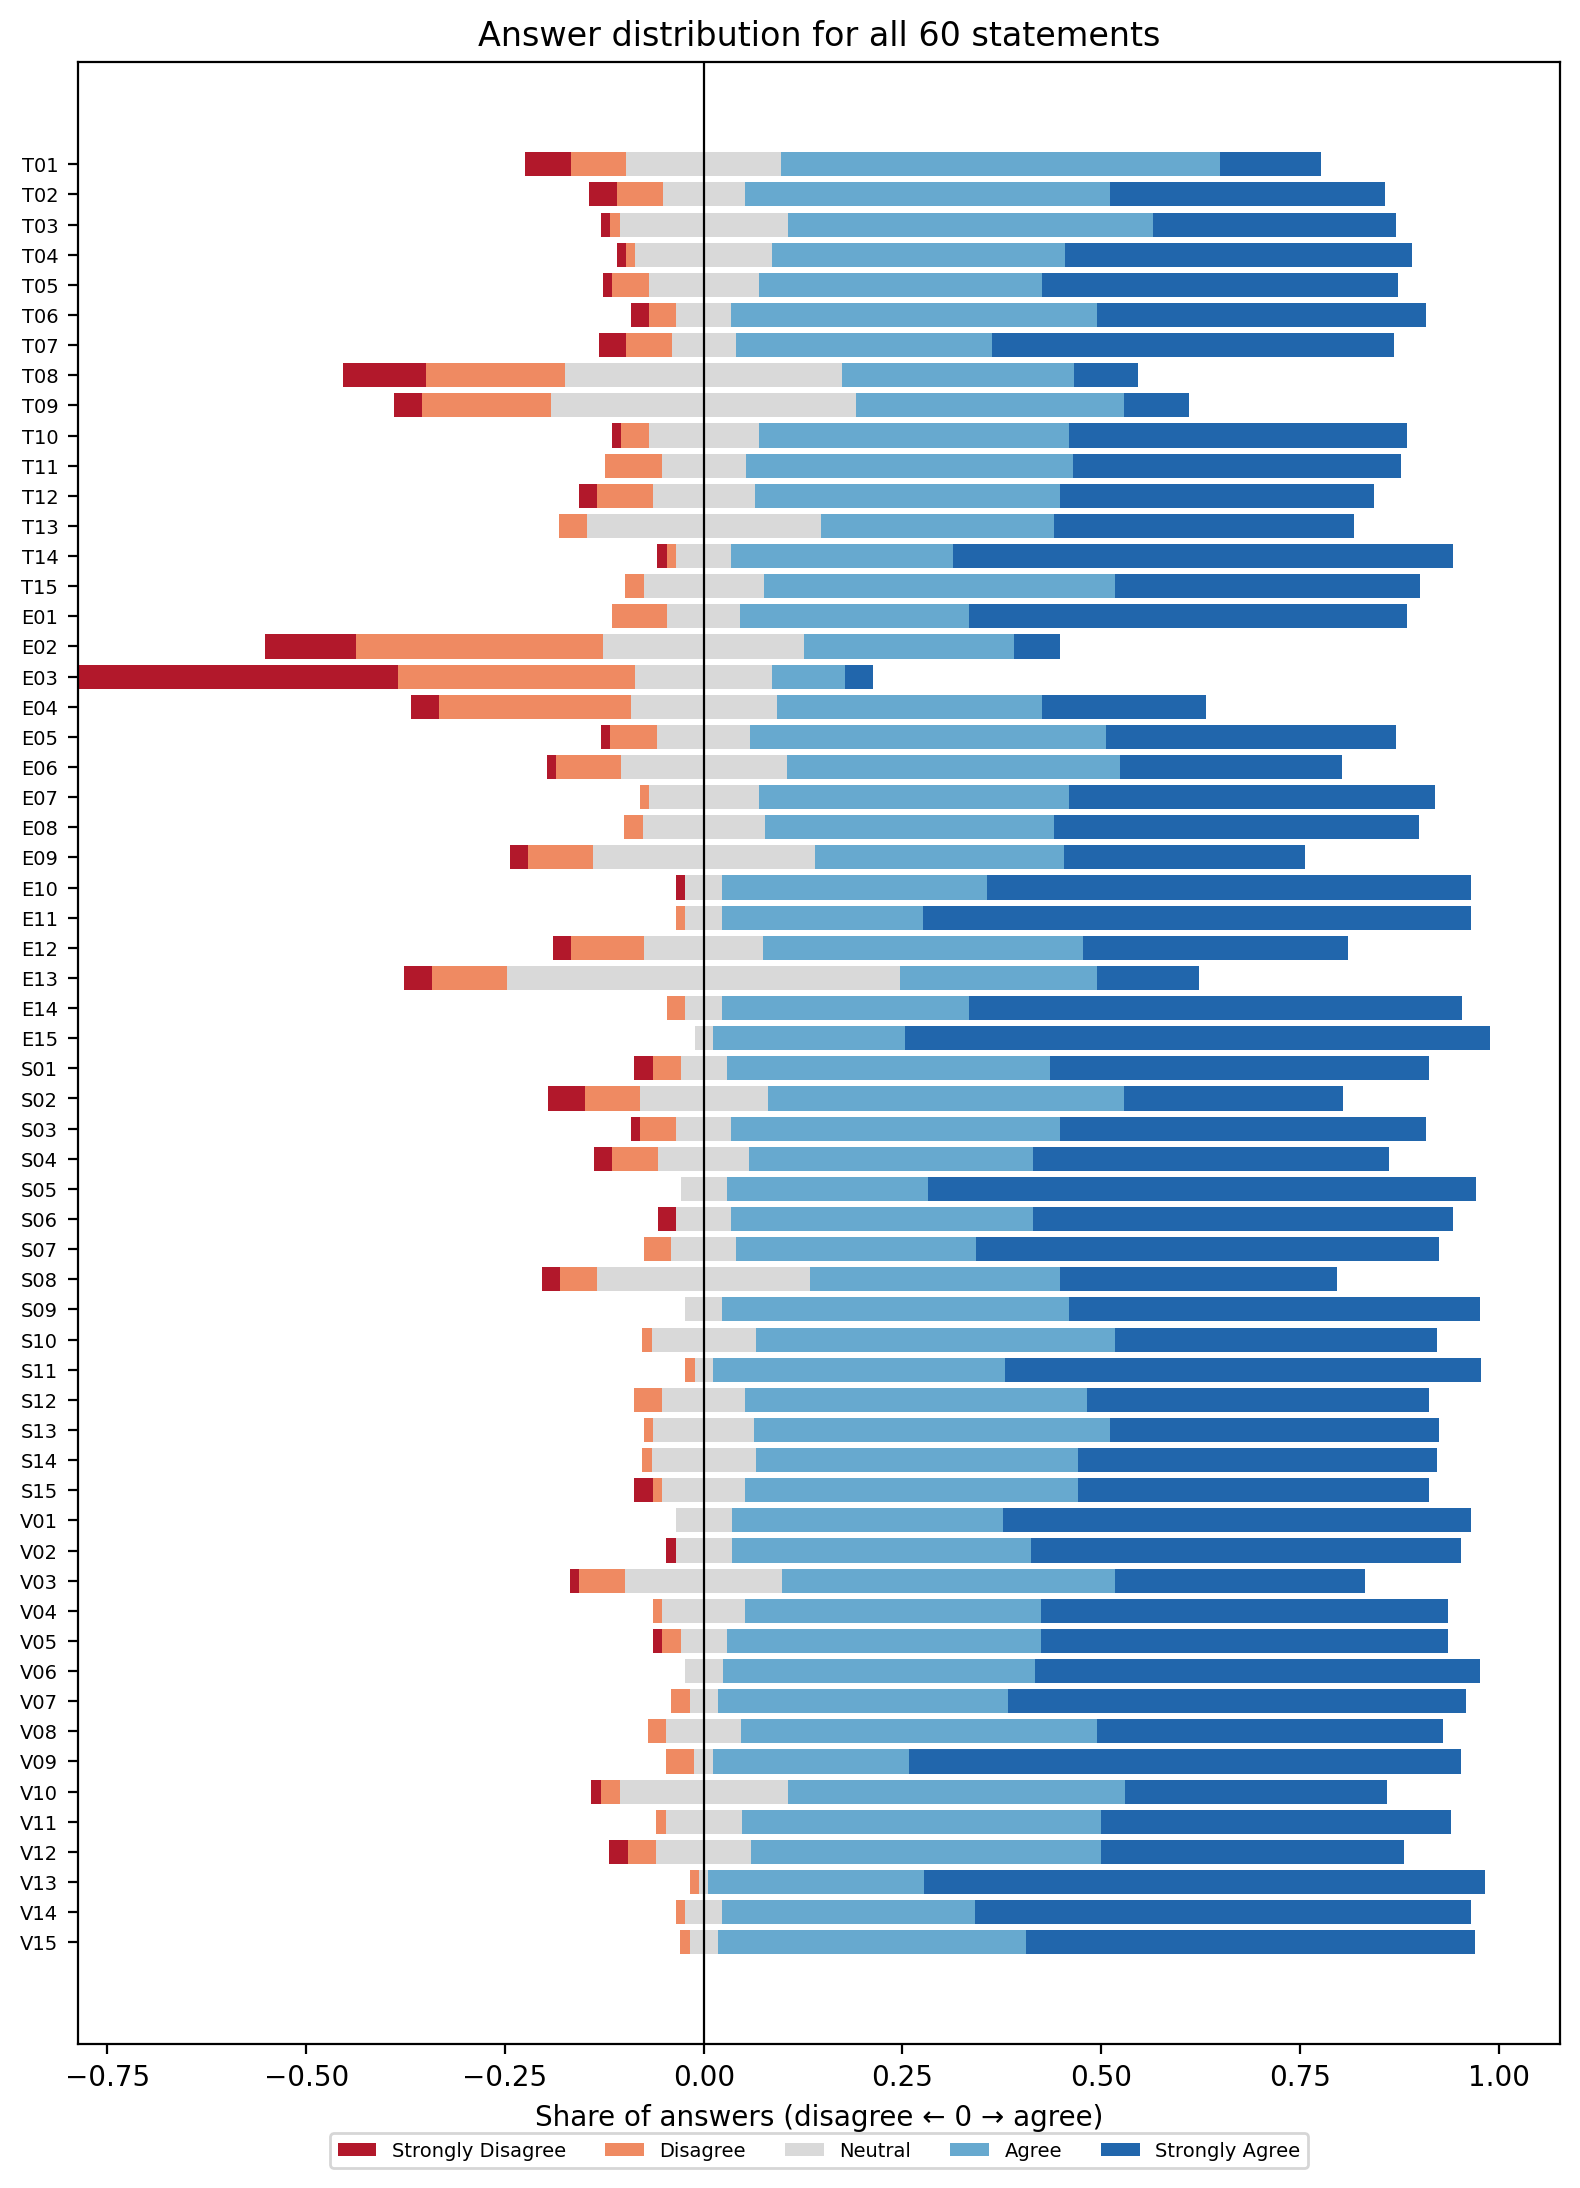
\includegraphics[width=\linewidth]{figures/fig1_answer_distribution.png}
\caption{Answers to all 60 statements: disagreement left, agreement right.}\label{fig:dist}
\end{minipage}\hfill
\begin{minipage}{0.53\linewidth}\centering
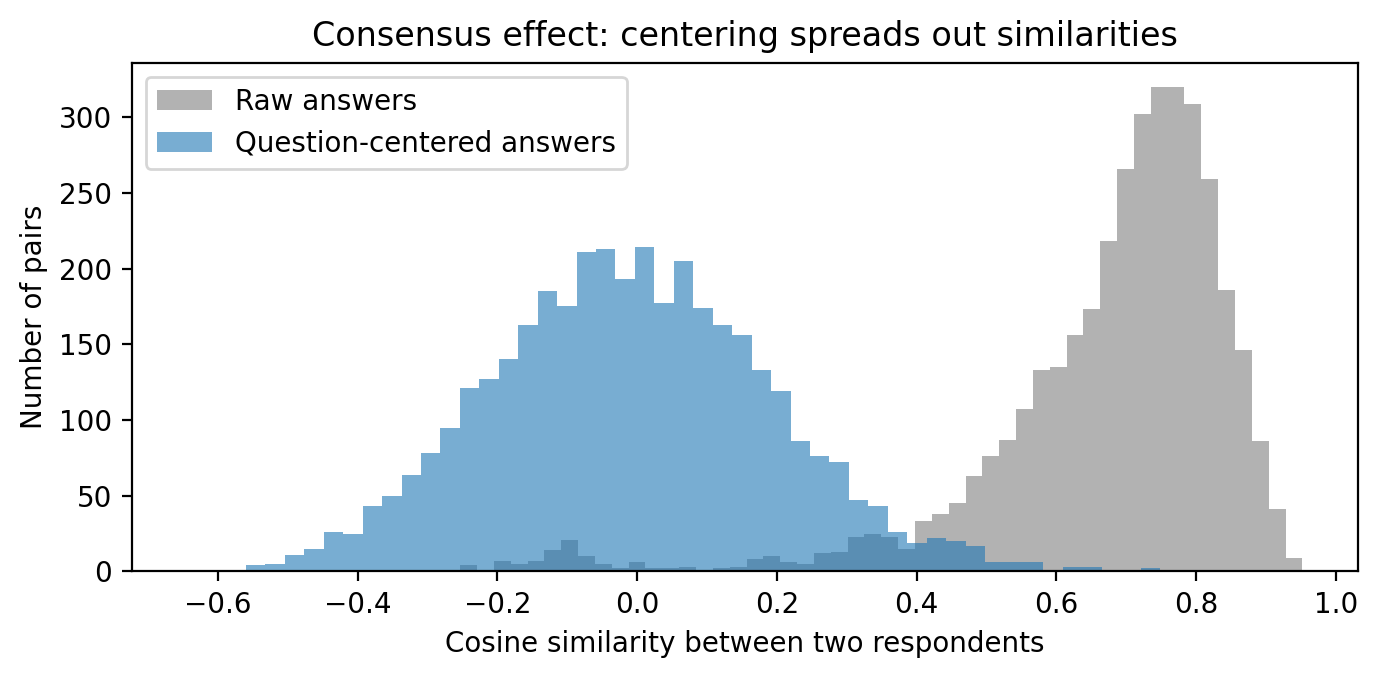
\includegraphics[width=\linewidth]{figures/fig3_similarity_centering.png}
\caption{Similarity between every pair of students before (grey) and after (blue) centring each statement.}\label{fig:center}
\vspace{6pt}
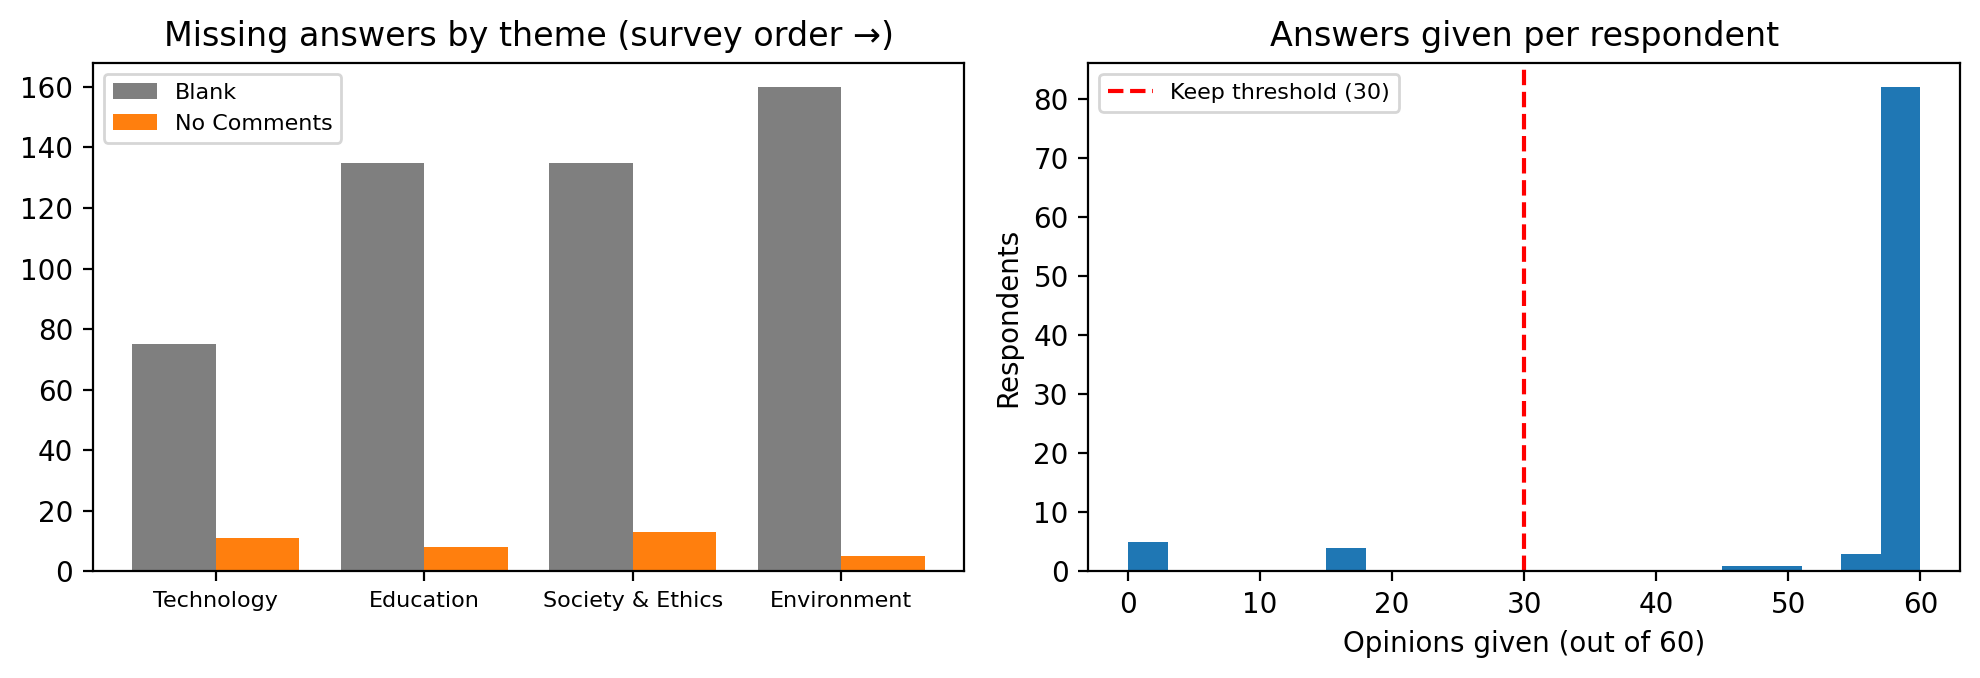
\includegraphics[width=\linewidth]{figures/fig2_missingness.png}
\caption{Missing answers by theme (left) and answers given per student, with the cut-off of 30 (right).}
\end{minipage}
\end{figure}

\section{Pipeline Followed}
We build three kinds of network. The respondent network (main) has the 87 students as nodes and undirected, weighted edges between students with similar opinions; it asks which students think alike. Four theme networks use the same method on 15 statements each; they ask whether one topic divides the class more than another. The belief network has the 60 statements as nodes, linked when answers to them are correlated; it asks which opinions go together.

\subsection{Step 1: centre each statement}
We subtract the class mean from every answer, $x'_{iq} = x_{iq}-\bar x_q$ \app{centring}. A value now says whether a student agrees more or less than the class. On E15 (mean $+1.71$) Strongly Agree becomes $+0.29$, close to zero, because nearly everyone said it. On E03 (mean $-0.94$) Agree becomes $+1.94$, because that student is unusual.

\subsection{Step 2: similarity}
For each pair we compute cosine similarity of the centred vectors \app{cosine} on statements both answered (at least 20 shared, otherwise 0). It is $+1$ when two students differ from the class in the same way and $-1$ when they differ in opposite ways. Fig.~\ref{fig:center} shows why Step 1 matters: on raw answers the mean similarity is $0.68$ and 22\% of pairs exceed $0.8$; after centring the mean is about 0 and similarities spread from $-1$ to $+1$.

\subsection{Step 3: edges}
Linking every positive pair would connect half the class. Instead each student is linked to their 6 most similar classmates ($k$-nearest neighbours) \app{knn}; edge A--B exists if either is in the other's top 6, weighted by similarity. This gives 366 edges and nobody is left isolated. We also test $k=4,5,8,10$, a top-10\% cut-off and a disparity-filter backbone \app{backbone}.

\subsection{Step 4: analyse}
Global metrics against random graphs; Louvain communities tested against two null models; profiles of each group; a response-style check; nine alternative pipelines; the theme and belief networks.

\section{Analysis and Visualizations}
\subsection{Global structure}
\begin{table}[H]\centering\small
\begin{tabular}{lll}\toprule
Metric & Value & Comparison\\\midrule
Nodes, edges, density & 87, 366, 0.098 \app{degree} & \\
Mean / max degree; components & 8.4 / 18; 1 & nobody is cut off\\
Average clustering & 0.242 & random 0.096, degree-preserving $0.098\pm0.009$\\
Average path length; diameter & 2.50; 4 & random 2.31\\
Small-world $\sigma$ & 2.31 & $>1$ means small-world\\
Degree assortativity & 0.086 \app{degassort} & near 0: no hub preference\\
Louvain modularity $Q$ & 0.452 & 5 communities\\\bottomrule
\end{tabular}\caption{Global metrics of the respondent network.}\end{table}

Clustering is 2.5 times that of a random graph with the same size \app{smallworld}, while paths are almost as short. Similarity is transitive: if A resembles B and B resembles C, A and C are usually alike, as expected when answers come from shared underlying attitudes. The network is a small world with a single component, so no group of students is isolated.

\subsection{Communities and null models}
Louvain finds five groups ($Q=0.452$) \app{louvain}. Any network has some modularity, so we test it two ways. (1) Shuffling each statement's answers across students 200 times \app{shufflenull} keeps every statement's answer distribution but breaks each student's pattern; rebuilt networks give $Q=0.406\pm0.015$ ($z=3.0$, none of 200 reached the real value) and clustering $0.153$ ($z=6.0$). (2) Rewiring the real network 100 times while keeping every degree \app{rewire} gives $Q=0.289\pm0.009$ against a real unweighted $0.422$ ($z=14.1$) and clustering $0.098$ ($z=15.3$). The groups are real, but the modest gap in test (1) means they overlap. Over 50 Louvain seeds the mean ARI is 0.62 \app{stability} (min 0.26): group cores are stable, border students move.

\begin{figure}[H]\centering
\begin{minipage}{0.46\linewidth}\centering
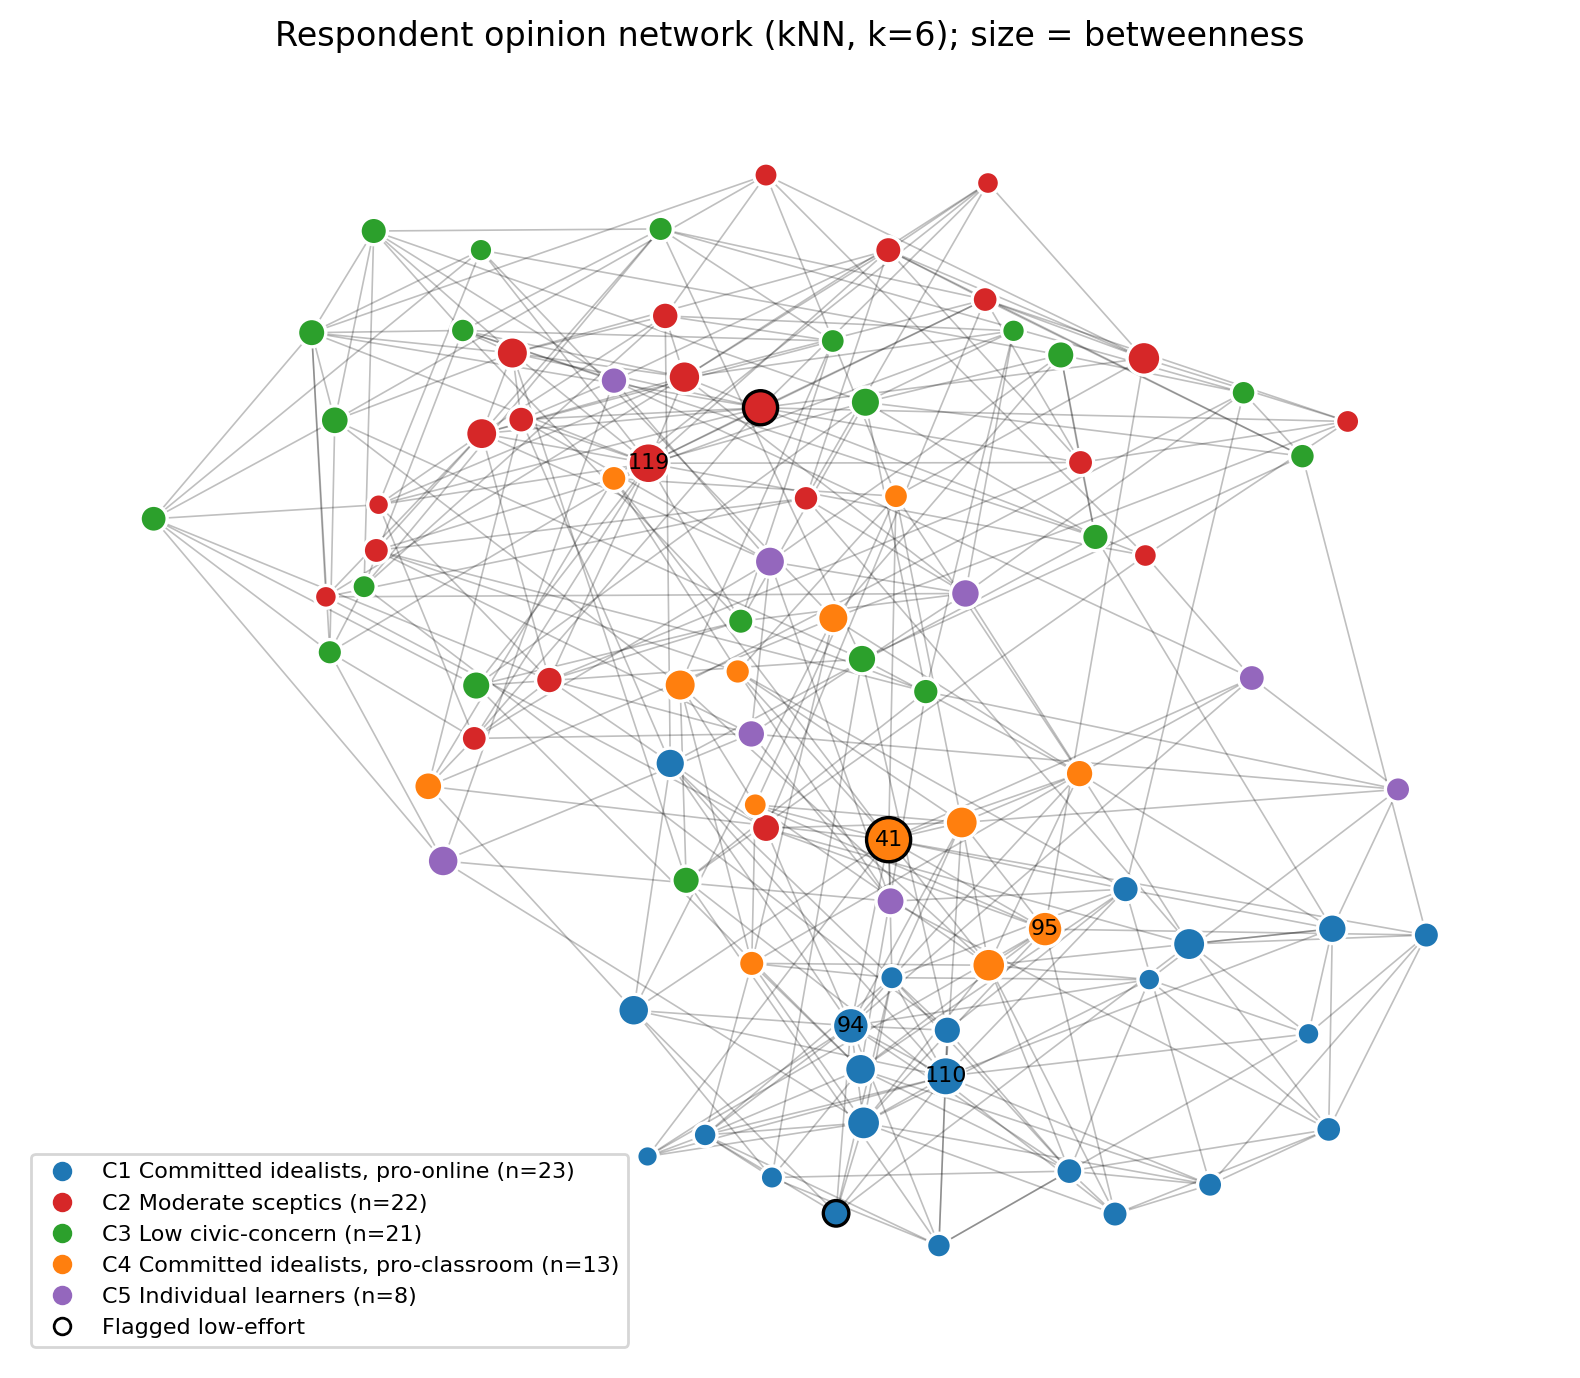
\includegraphics[width=\linewidth]{figures/fig4_respondent_network.png}
\caption{Respondent network. Colour = group, size = betweenness, black ring = flagged student.}\label{fig:net}
\end{minipage}\hfill
\begin{minipage}{0.52\linewidth}\centering
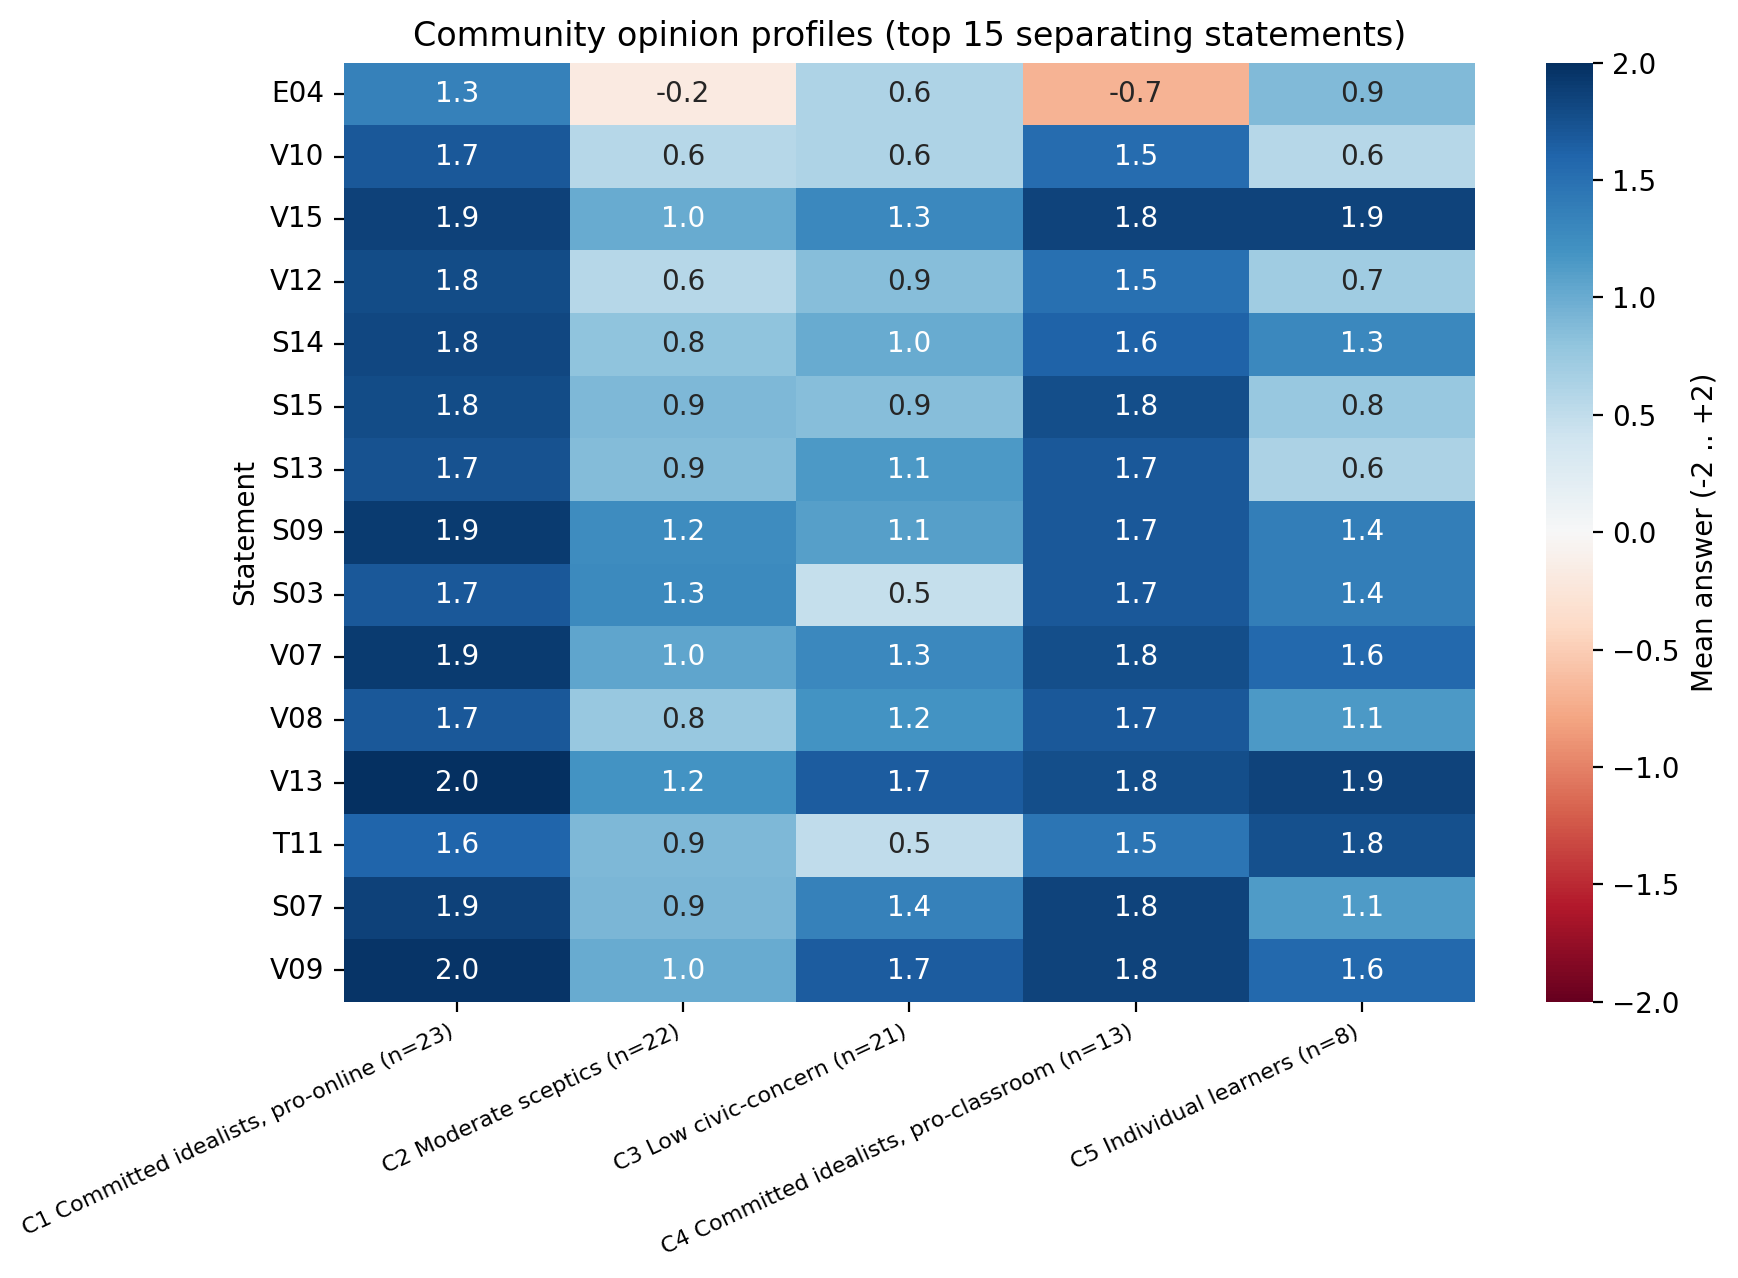
\includegraphics[width=\linewidth]{figures/fig6_community_heatmap.png}
\caption{Mean answer of each group on the 15 statements that separate groups most (Kruskal--Wallis $\varepsilon^2$) \app{kruskal}.}\label{fig:heat}
\end{minipage}
\end{figure}

\begin{figure}[H]\centering
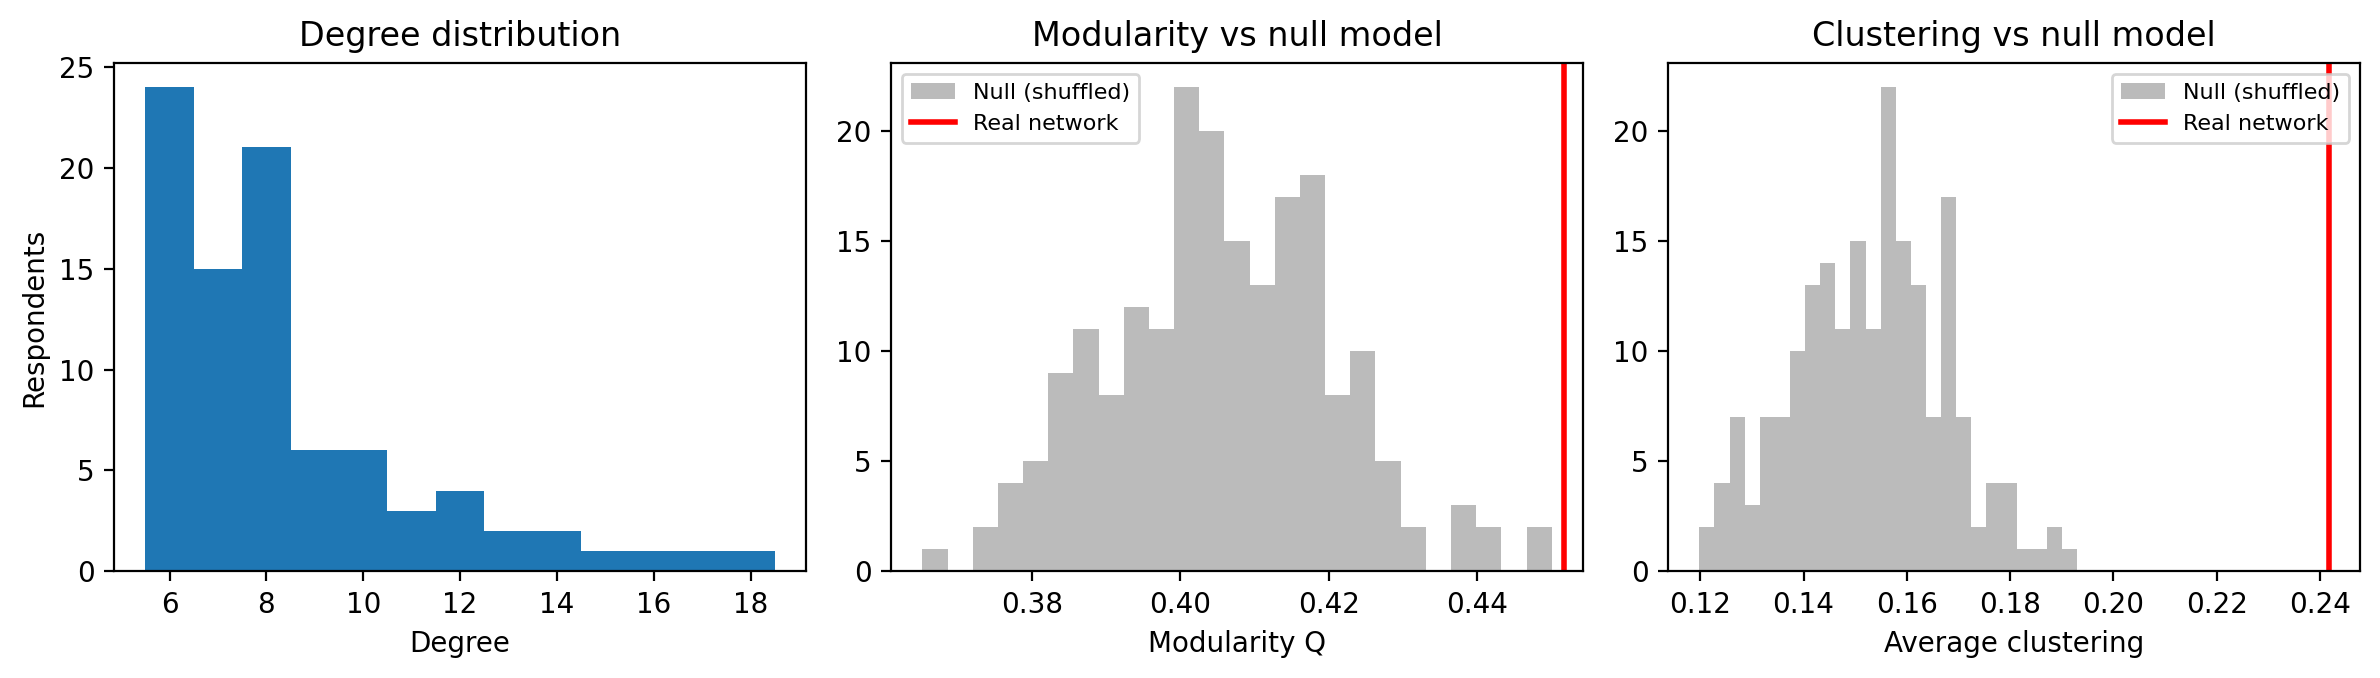
\includegraphics[width=0.9\linewidth]{figures/fig5_degree_null.png}
\caption{Degree distribution, and real modularity and clustering (red) against 200 shuffled-data networks.}\label{fig:null}\end{figure}

\subsection{What each group believes}
\begin{table}[H]\centering\small
\begin{tabularx}{\linewidth}{l c X}\toprule
Group & $n$ & What sets it apart (Fig.~\ref{fig:heat})\\\midrule
C1 Committed idealists, pro-online & 23 & Strongest agreement on society, environment and ethics; strongly back online learning (E04 $+1.3$)\\
C2 Moderate sceptics & 22 & Mild agreement on nearly everything; slightly against online learning (E04 $-0.2$)\\
C3 Low civic concern & 21 & Lowest on reviewing tech's social impact (S03), algorithm transparency (T11), civic duty (S01) and collaboration (E09)\\
C4 Committed idealists, pro-classroom & 13 & Same strong values as C1 but against online learning (E04 $-0.7$)\\
C5 Individual learners & 8 & Prefer learning alone (E09 $+0.1$); links spread across groups (participation coefficient 0.64)\\\bottomrule
\end{tabularx}\caption{The five groups of the respondent network.}\end{table}
The strongest bridges (highest betweenness on distance $1-$similarity) \app{centrality} are students 41, 119, 110 and 94. C1 is the most inward-looking group (participation 0.36).

\subsection{Intensity or content?}
In Fig.~\ref{fig:heat}, C1 and C4 are dark blue almost everywhere and C2 and C3 lighter almost everywhere. This could mean the groups hold different beliefs, or it could mean some students habitually tick ``Strongly Agree'' where others tick ``Agree'' (survey researchers call this response style). Two checks point to response style. Assortativity by each student's mean answer is $+0.65$ \app{attrassort}: students link to others with the same overall level. In a PCA of the centred answers \app{pca}, PC1 explains 17.2\% of the variance (PC2 6.2\%), 95\% of its loadings share a sign, and PC1 scores correlate $0.98$ with the mean answer.

We therefore rebuilt the network with Pearson correlation \app{pearson}, which also removes each student's own mean, so only the ranking of topics counts. Assortativity by mean answer falls to $0.16$, yet structure remains ($Q=0.455$ vs $0.405\pm0.016$, $z=3.2$) with seven groups that barely overlap the first five (ARI 0.27). Seven of the nine statements separating them are about education (Fig.~\ref{fig:pheat}): P1 traditionalists (the only group backing compulsory attendance and exams), P4 classroom reformers (against attendance rules and online learning), P3 online and collaborative learners, P6 exam-backing individualists, and P7 progressive regulators (strongest against exams and attendance, strongest for AI regulation and data protection).

\begin{figure}[H]\centering
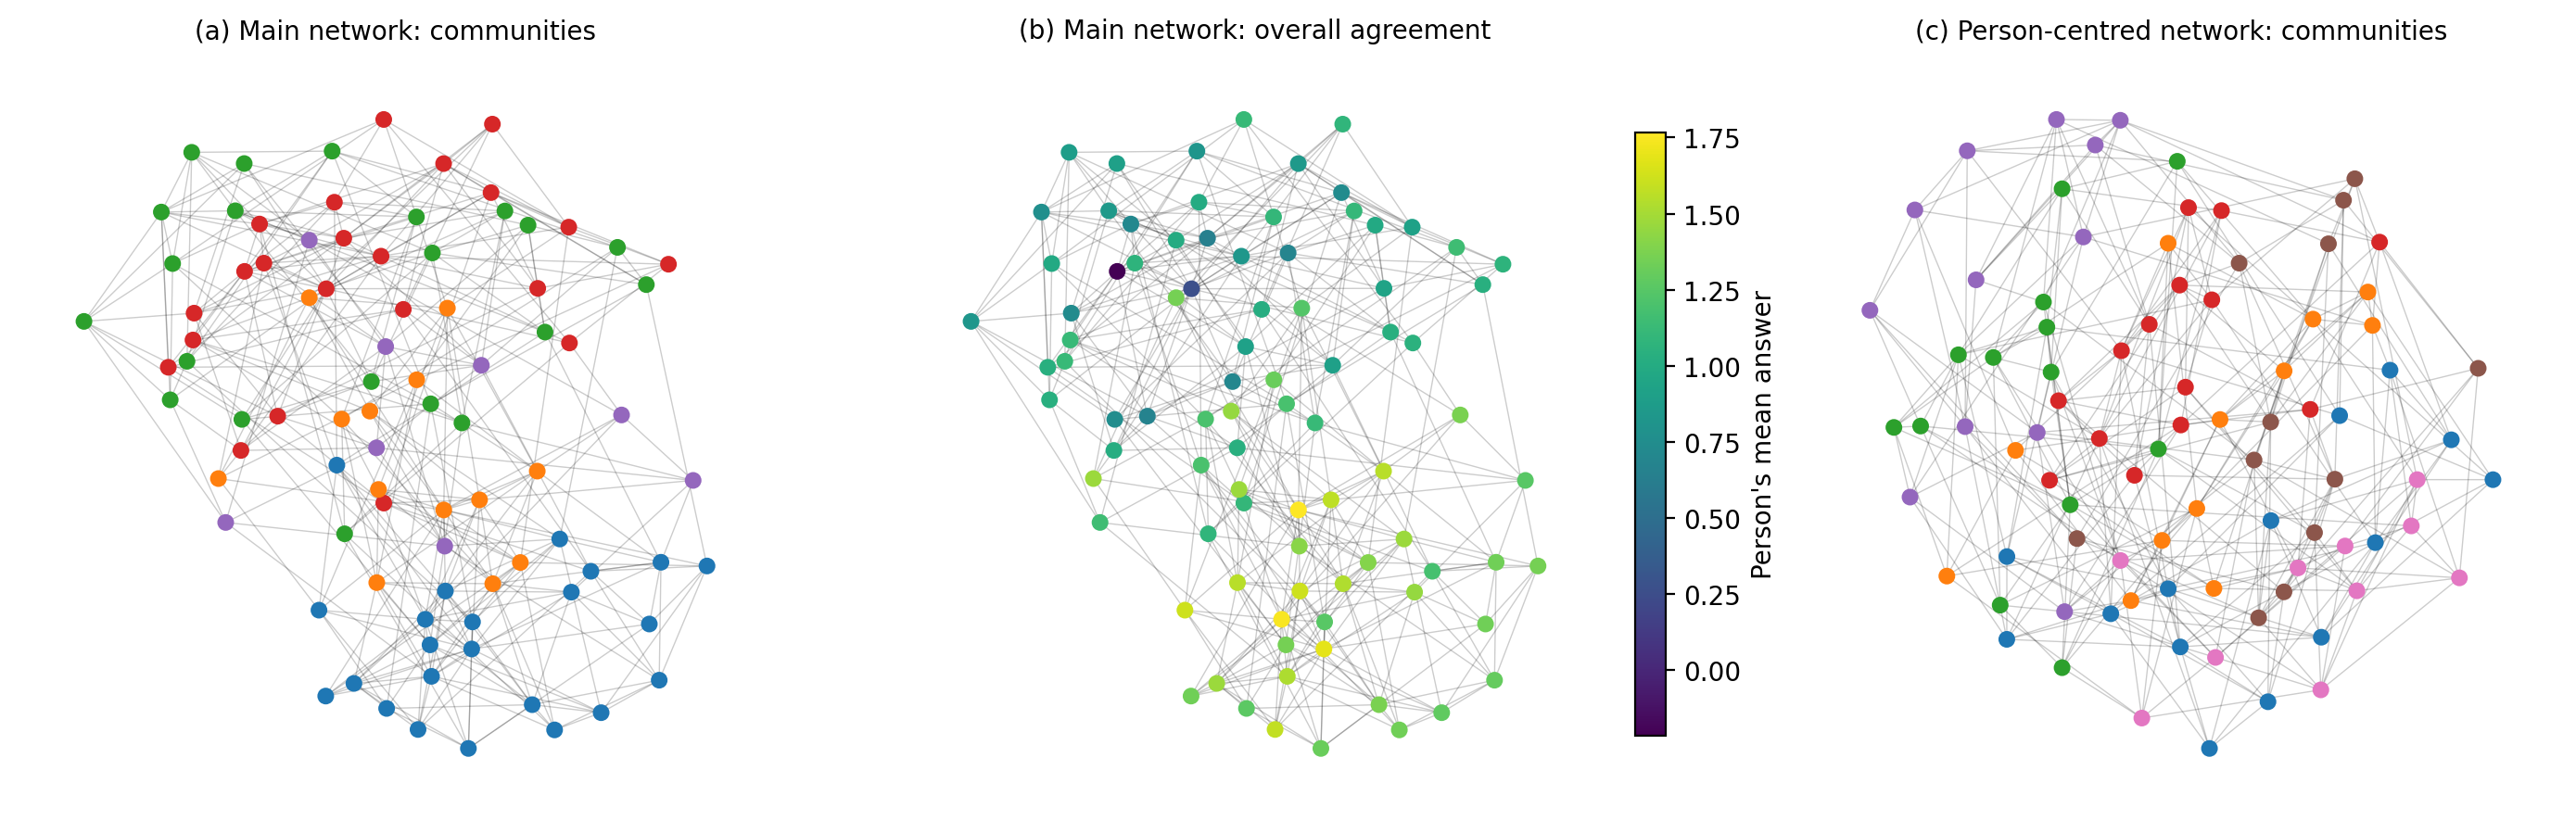
\includegraphics[width=0.95\linewidth]{figures/fig11_intensity.png}
\caption{(a) Groups of the main network. (b) Same layout coloured by each student's mean answer: groups follow the agreement gradient. (c) Groups of the Pearson network.}\label{fig:int}
\end{figure}
\begin{figure}[H]\centering
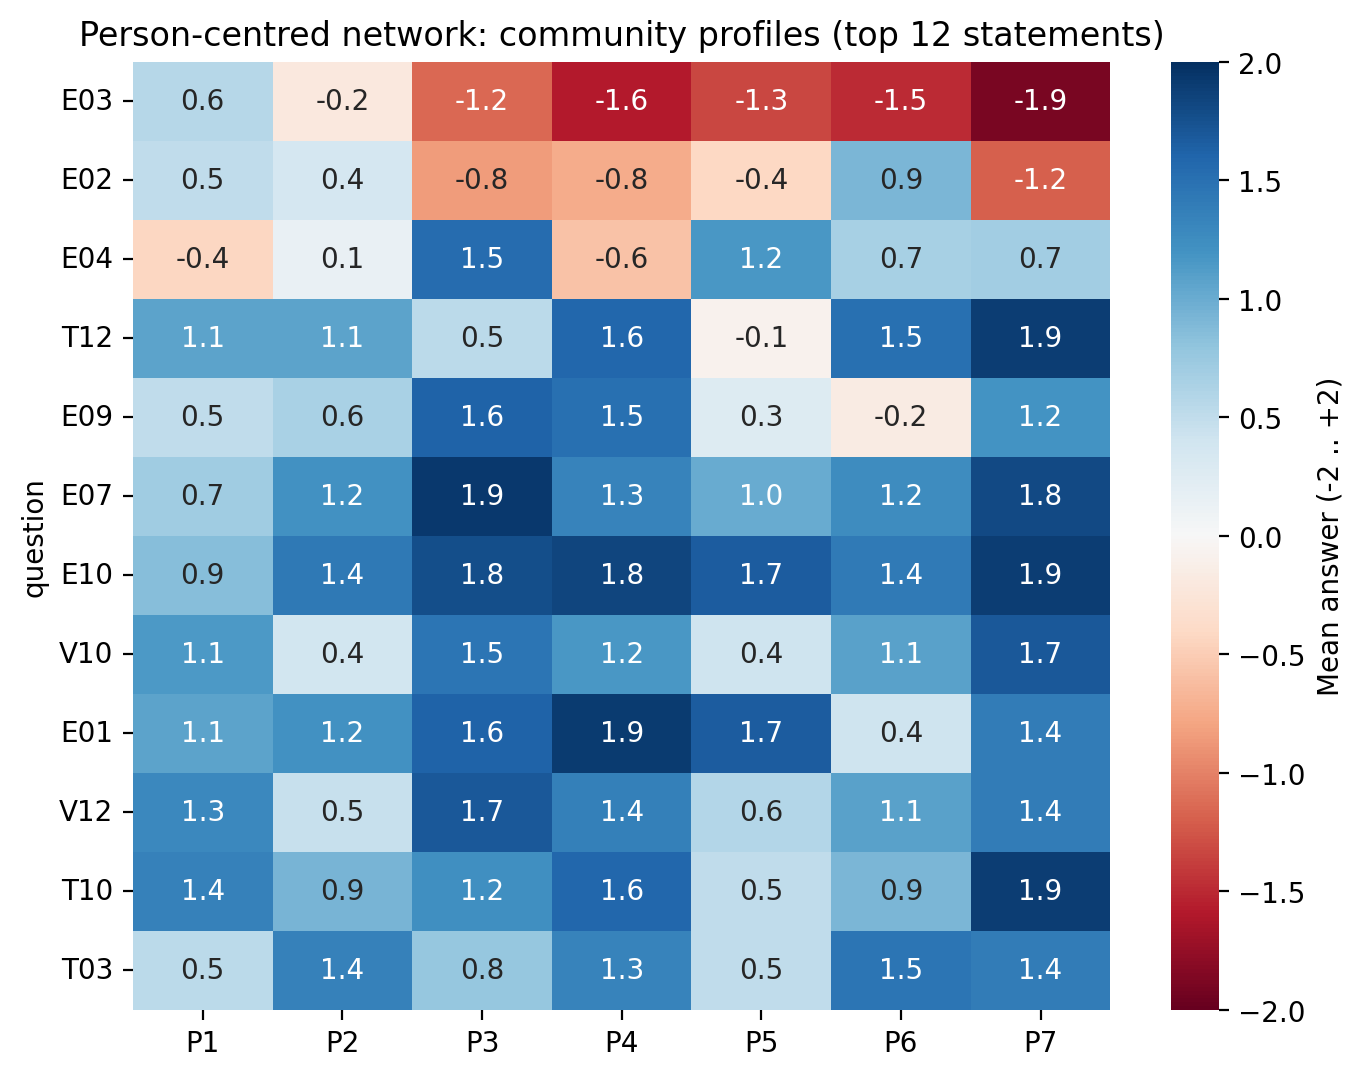
\includegraphics[width=0.55\linewidth]{figures/fig12_pearson_heatmap.png}
\caption{Pearson groups on their 12 most separating statements.}\label{fig:pheat}
\end{figure}

\subsection{Robustness}\label{sec:rob}
\begin{table}[H]\centering\small
\begin{tabular}{lrrrrr}\toprule
Version & Edges & $Q$ & Groups & ARI & NMI\\\midrule
kNN $k=4$ & 259 & .51 & 6 & .53 & .63\\
kNN $k=5$ & 317 & .47 & 6 & .61 & .68\\
kNN $k=8$ & 466 & .42 & 4 & .48 & .61\\
kNN $k=10$ & 563 & .40 & 2 & .39 & .52\\
Top 10\% of similarities & 178 & .49 & 7 & .38 & .59\\
Disparity backbone & 30 & .91 & 16 & .23 & .62\\
Pearson similarity & 324 & .45 & 7 & .27 & .46\\
No centring & 467 & .28 & 6 & .07 & .22\\
Without 3 flagged students & 346 & .43 & 5 & .58 & .69\\\bottomrule
\end{tabular}\caption{Alternative pipelines compared with the main partition \app{arinmi}.}\end{table}
Nearby choices keep most of the structure (NMI 0.61 to 0.69 for $k=4$ to 8 and without flagged students). Without centring the groups nearly vanish (ARI 0.07), which confirms Step 1. The Pearson version differs because it removes intensity (Section 5.4). The backbone keeps 30 edges in 16 pieces, so its $Q$ is not comparable.

\subsection{Theme networks}
\begin{table}[H]\centering\small
\begin{tabular}{lrrrrr}\toprule
Theme & Mean answer & Polarization & $Q$ & Shuffled $Q$ & $z$\\\midrule
Technology & 1.00 & 0.21 & 0.486 & 0.485 & 0.06\\
Education & 0.91 & 0.22 & 0.501 & 0.490 & 0.58\\
Society \& Ethics & 1.28 & 0.12 & 0.503 & 0.500 & 0.16\\
Environment & 1.39 & 0.08 & 0.496 & 0.481 & 0.76\\\bottomrule
\end{tabular}\caption{Per-theme networks against their own null models (polarization $=4\times$ share agreeing $\times$ share disagreeing \app{polar}).}\end{table}
Education and Technology have the most disagreement; Environment has almost none. Yet no theme network has structure beyond chance (all $z<1$), and groups from different themes barely match (NMI 0.09 to 0.17, Fig.~\ref{fig:theme}). Two students who agree about AI are no more likely than others to agree about education. Clear groups appear only when all 60 statements are combined.

\begin{figure}[H]\centering
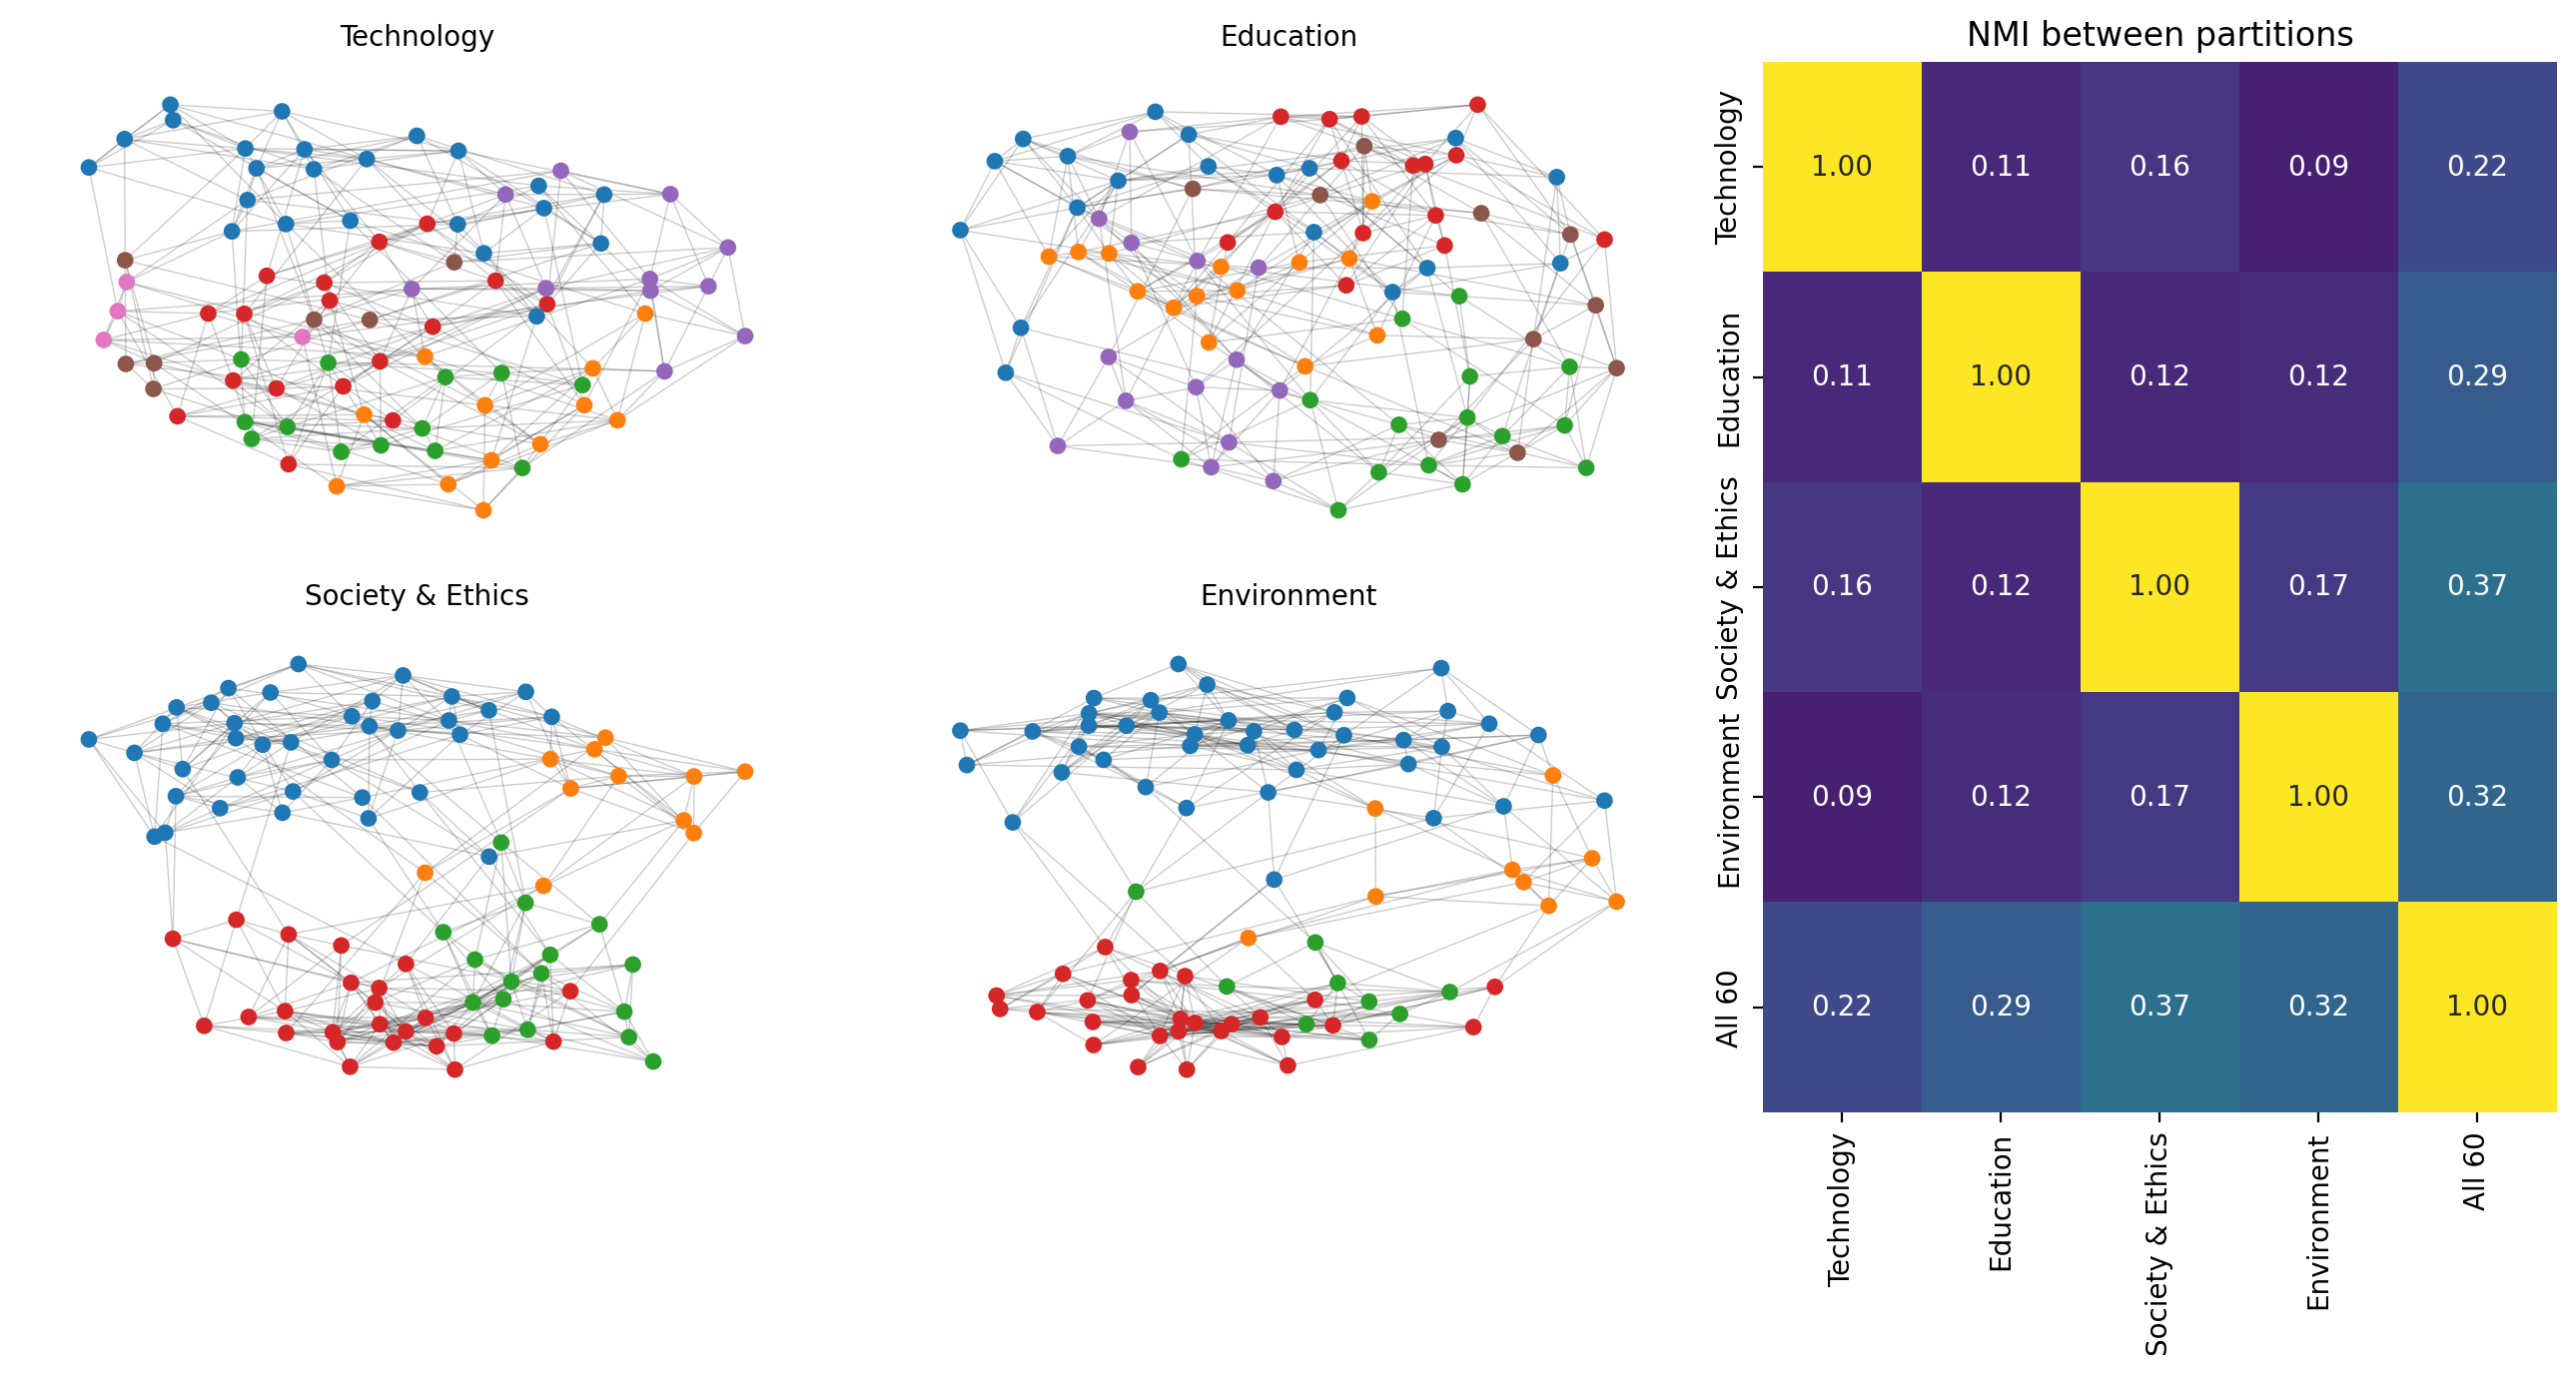
\includegraphics[width=0.85\linewidth]{figures/fig7_theme_networks.png}
\caption{Theme networks (colour = each theme's own groups) and NMI between all partitions.}\label{fig:theme}\end{figure}

\subsection{Belief network}
Nodes are the 60 statements; an edge joins two statements whose Spearman correlation \app{spearman} is significant after Benjamini--Hochberg FDR correction \app{fdr} ($q<0.05$), keeping its sign. The network has 431 edges (density 0.244), only 10 of them negative. 44\% of edges are within a theme against 24\% expected at random, and Louvain's clusters match the survey themes only partly (NMI 0.51) while splitting the network better ($Q=0.206$ vs $0.154$). The clusters are education reform with AI in education, environment, society and ethics, and technology risk and regulation with data privacy. The most connected statements are S09 (respectful discussion), S14 (ethical leadership), V15 (future generations) and S06 (shared fight against misinformation). Nearly every negative edge involves E03 or E02, forming a traditional-versus-progressive education axis (E03 vs E10, $\rho=-0.41$). All 1{,}560 triangles are structurally balanced \app{balance}, against 93.4\% with shuffled signs.

\begin{figure}[H]\centering
\begin{minipage}{0.5\linewidth}\centering
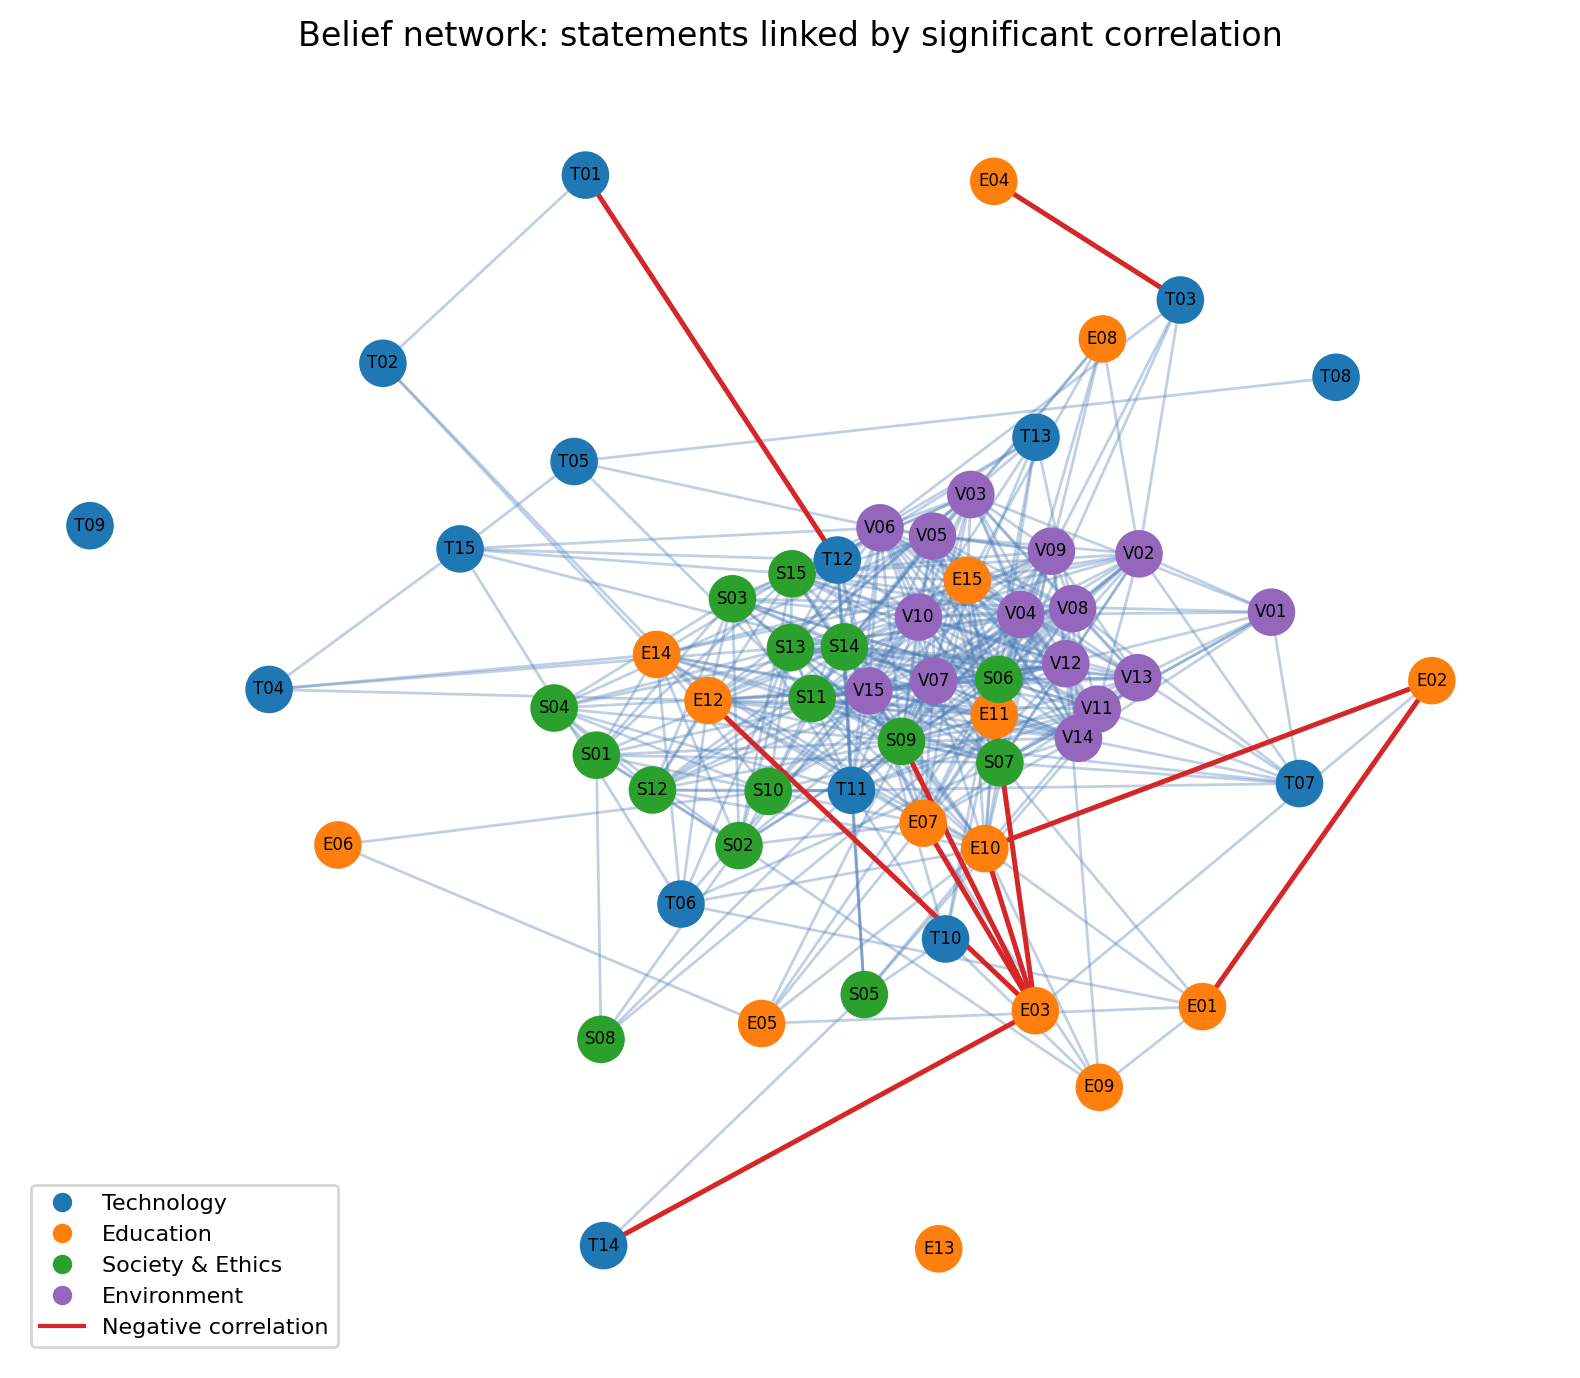
\includegraphics[width=\linewidth]{figures/fig8_statement_network.png}
\caption{Belief network: colour = theme, red edges = negative correlation.}
\end{minipage}\hfill
\begin{minipage}{0.47\linewidth}\centering
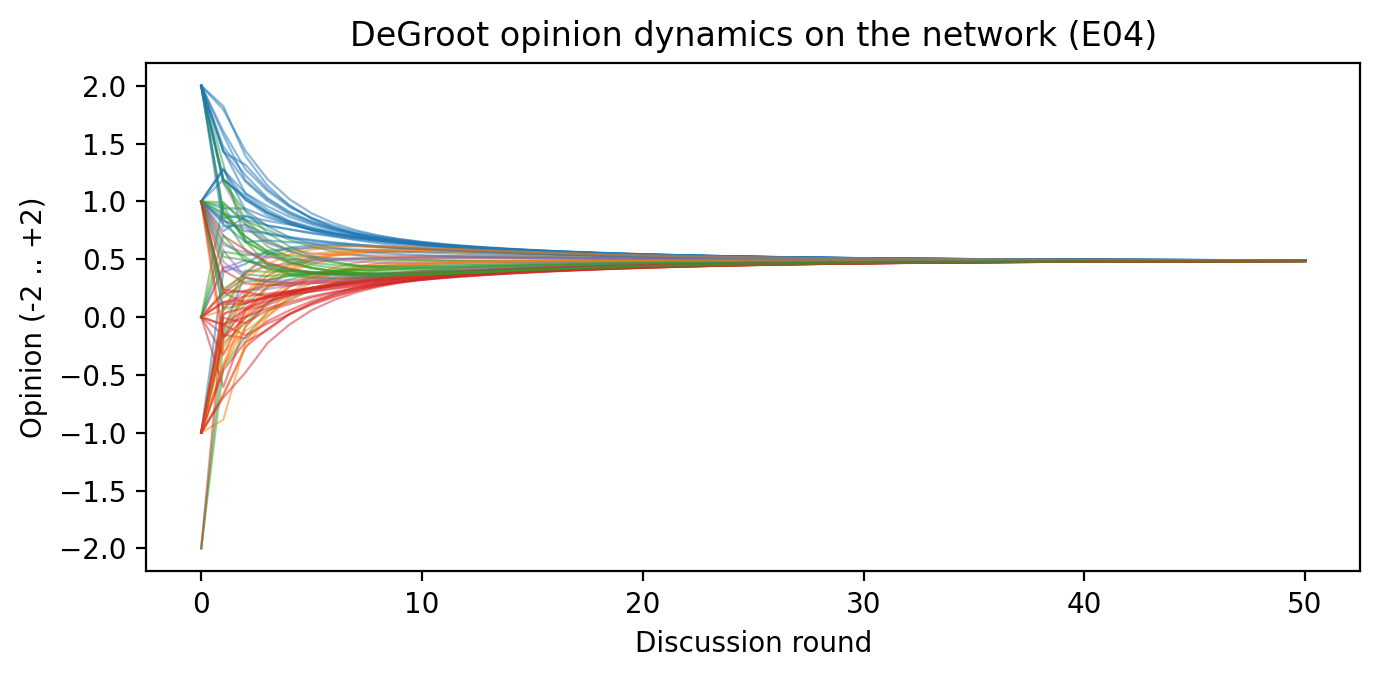
\includegraphics[width=\linewidth]{figures/fig10_degroot.png}
\caption{DeGroot opinion trajectories on E04 (colour = group).}\label{fig:dg}
\end{minipage}
\end{figure}

\subsection{Opinion dynamics}
We ran a DeGroot model on E04 \app{degroot} (online learning), the most polarized statement: each round every student takes a similarity-weighted average of their own and their neighbours' opinions. The standard deviation falls from 1.16 to 0.21 in five rounds, and the final opinion ($+0.49$) sits near the class mean ($+0.44$), so no group dominates (Fig.~\ref{fig:dg}). Our edges are similarities between answers, and we do not know who actually talks to whom, so the simulation only shows what could happen if students discussed along these links.

\section{Results and Discussion}
\begin{enumerate}
  \item The class mostly agrees. 79\% of answers are agreement, and the disagreement that exists is mainly about education (attendance, exams, online learning), with some about technology.
  \item On raw answers nearly everyone looks alike. After centring each statement, five groups appear that beat both null models ($z=3.0$ and $14$). They overlap, and students at their borders change group between runs.
  \item The strongest difference between students is how strongly they agree. Students link to others with the same overall agreement level (assortativity $0.65$), and PC1 is almost the same as each student's mean answer ($r=0.98$). Some of this may be conviction and some answering habit. We think any opinion network built from Likert data should test for it.
  \item With each student's overall level removed, seven groups remain and still beat chance ($z=3.2$). Education statements separate them most.
  \item Opinions depend on the topic. No single theme produces groups beyond chance, and the groups found in different themes barely match.
  \item The belief system is consistent. Statements group by worldview more than by survey section, civic values sit at the centre, the only real opposition is traditional versus progressive education, and every triangle is balanced.
  \item In the DeGroot model, disagreement on online learning shrinks by over 80\% in five rounds.
\end{enumerate}
\subsection*{Limitations}
The sample is small (87 students). We treat Likert answers as equally spaced, and use rank-based tests where possible to reduce the effect of this assumption. Our edges measure similarity of answers and say nothing about who talks to whom. Group membership shifts with $k$, the similarity measure and the random seed (Section 5.5), so we only claim results that hold across versions. Because most answers are agreement, there is little variation at the top of the scale, and more answers are missing late in the survey.

\section{Individual Contribution}
\begin{table}[H]\centering\small
\begin{tabularx}{\linewidth}{l X c}\toprule
Member & Tasks completed & Share\\\midrule
Vedant Pahariya (2023112012) & Survey parsing and Likert encoding, missing-data analysis and the 30-answer cut-off, careless-answer flags (\texttt{data\_prep.py}); answer-distribution and missingness figures (Figs.\ 1, 3); theme networks with their own null models and the polarization index; Sections 3 and 5.6 of the report & 33\%\\
Siddhant Gudwani (2024102042) & Item centring, cosine and Pearson similarity, kNN, threshold and backbone networks (\texttt{network.py}); both null models (shuffled and degree-preserving); community detection, seed stability and group profiles; intensity analysis (assortativity, PCA, Pearson network); Sections 4, 5.2 to 5.4 of the report & 34\%\\
Krishna Goel (2023112009) & Global metrics and small-world test; robustness study over nine alternative pipelines; belief network with FDR edges, theme match and structural balance; DeGroot simulation; their figures (\texttt{plots\_results.py}), pipeline script (\texttt{run\_all.py}) and README; Sections 5.1, 5.5, 5.7, 5.8, 6 and the Appendix & 33\%\\\bottomrule
\end{tabularx}\end{table}
AI tools, which the assignment allows, helped write code and draft text; the team checked every result.

%==================================================================
\newpage
\appendix
\section*{Appendix: Techniques used, explained}
\small
This appendix explains every method in the report from the basics, in the order it is used.
\begin{multicols}{2}

\tech{Likert encoding}{likert} A Likert item has an order (Agree is more than Neutral) but no guaranteed spacing: we cannot be sure the step from Neutral to Agree equals the step from Agree to Strongly Agree. Most survey analyses still treat the steps as equal, because it lets us use averages and similarity measures. To make sure our conclusions do not depend on this assumption, we also use tests that only look at the order of answers (Spearman correlation and the Kruskal--Wallis test, explained later).

\tech{Mean-centring}{centring} Subtracting a column's average from every value in that column. It moves the ``typical'' answer to zero, so every number now describes how far a person is from the typical answer. It does not change how students are ordered on any one statement.

\tech{Cosine similarity}{cosine} Think of each student as an arrow in a 60-dimensional space, one direction per statement. Cosine similarity is the cosine of the angle between two arrows. It looks at the direction of the arrows and ignores their length. So it asks ``do these two students lean the same way?'' and does not care how strongly each one leans.

\tech{$k$-nearest-neighbour (kNN) graph}{knn} Each node is joined to the $k$ nodes most similar to it. The alternative is a single global cut-off (for example ``link all pairs above 0.3''). A global cut-off can leave students with unusual views with no edges at all, and they would drop out of the analysis. kNN guarantees every student at least $k$ links. We chose $k = 6$, close to the common rule of thumb $k \approx \ln N$ ($\ln 87 \approx 4.5$) rounded up for a connected graph, and we test $k = 4, 5, 8, 10$ in Section 5.5.

\tech{Disparity-filter backbone (used as a check)}{backbone} A different way to pick edges. For each student, it asks whether an edge is stronger than it would be if that student's total similarity were split at random over all their edges. For a node with $k$ edges and total weight $s$, an edge of weight $w$ has
\[ p = \left(1 - \frac{w}{s}\right)^{k-1}, \]
and the edge is kept if $p < 0.05$. It keeps only edges that are surprisingly strong. We use it, together with a ``top 10\% of all similarities'' cut-off, to check that our results do not depend on the kNN rule.

\tech{Degree, density and components}{degree} The degree of a node is how many edges it has. Density is the number of edges divided by the number of possible edges. A connected component is a set of nodes that can all reach each other; one component means nobody is cut off.

\tech{Clustering, path length and the small-world test}{smallworld} Clustering measures how often two neighbours of a node are also neighbours of each other (``are my friends' friends also my friends?''). It runs from 0 to 1. The average path length is the average number of steps on the shortest route between two nodes.

To judge whether these values are high or low, we compare them with an Erd\H{o}s--R\'enyi random graph that has the same number of nodes and edges but places the edges completely at random. A small-world network has much higher clustering than the random graph but a similar path length. We combine the two in one number,
\[ \sigma = \frac{C / C_{\text{random}}}{L / L_{\text{random}}}, \]
and a network with $\sigma > 1$ is called small-world.

\tech{Degree assortativity}{degassort} The correlation between the degrees of the two nodes at each end of an edge. A positive value means well-connected nodes tend to link to other well-connected nodes; a negative value means they tend to link to poorly connected ones; near 0 means no preference.

\tech{Modularity and the Louvain algorithm}{louvain} Modularity $Q$ scores how well a split of the network into groups keeps edges inside the groups:
\[ Q = \frac{1}{2m}\sum_{i,j}\left[A_{ij} - \frac{k_i k_j}{2m}\right]\delta(c_i, c_j). \]
Here $A_{ij}$ is the edge weight between $i$ and $j$, $k_i$ is the total weight of $i$'s edges, $m$ is the total weight in the network, and $\delta(c_i, c_j)$ is 1 if $i$ and $j$ are in the same group. In words: $Q$ is the share of edge weight inside groups minus the share we would expect if edges were placed at random while keeping each node's degree. $Q$ near 0 means no real groups; values above about 0.3 usually indicate clear groups.

Louvain is a fast method that searches for a split with high $Q$. It starts with every node in its own group, moves nodes into neighbouring groups whenever that raises $Q$, then merges each group into a single node and repeats. It uses randomness, so we ran it 20 times and kept the split with the highest $Q$.

\tech{Null model by shuffling each statement}{shufflenull} We shuffle the answers to each statement among the students, separately for every statement. After shuffling, each statement still has exactly the same number of Agree, Disagree and other answers, but a student's answer to one statement no longer has anything to do with their answer to another. We then build the network from the shuffled data with the exact same steps and record its modularity and clustering. We did this 200 times.

The $z$-score says how far the real value is from these shuffled values, measured in standard deviations:
\[ z = \frac{\text{real value} - \text{average of shuffled values}}{\text{standard deviation of shuffled values}}. \]
A $z$ above about 2 means the real value is very unlikely to come from chance.

\tech{Degree-preserving null (rewiring)}{rewire} A stricter test. We take the real network and repeatedly pick two edges, A--B and C--D, and swap their ends to get A--D and C--B. After many swaps (10 times the number of edges), every student still has exactly as many links as before, but who is linked to whom is random. If the real network still has more clustering and modularity than these rewired copies, the structure comes from who is linked to whom, and cannot be explained just by some students having more links than others. We made 100 rewired copies.

\tech{Stability of the groups across runs}{stability} Because Louvain uses randomness, we ran it 50 times with different seeds and compared every pair of results with the Adjusted Rand Index (ARI). ARI is 1 when two splits are identical and about 0 when they agree no more than random labelling would. We got a mean ARI of 0.62 and a minimum of 0.26.

\tech{Kruskal--Wallis test and effect size}{kruskal} For each statement, the Kruskal--Wallis test asks whether the groups answer it differently. It ranks all answers from lowest to highest and checks whether some groups have systematically higher ranks. It only uses the order of answers, so it does not rely on the equal-spacing assumption. The effect size $\varepsilon^2 = H \big/ \frac{n^2 - 1}{n + 1}$ (where $H$ is the test statistic and $n$ the number of answers) gives the share of variation in the answers that group membership explains, from 0 to 1. We rank statements by $\varepsilon^2$.

One caution: the groups were found from these same answers, so these tests describe the groups. They do not prove the groups exist; the null models do that.

\tech{False discovery rate (Benjamini--Hochberg)}{fdr} When we run 60 tests at the 5\% level, about 3 will come out ``significant'' by chance. The Benjamini--Hochberg correction adjusts the $p$-values so that, among all results we call significant, at most 5\% are expected to be false. We report corrected values throughout.

\tech{Betweenness, eigenvector centrality and participation coefficient}{centrality} Betweenness counts how many of the shortest routes between other students pass through a student. For this we treat $1 - \text{similarity}$ as the length of an edge, so very similar students are ``close''. A student with high betweenness sits between groups.

Eigenvector centrality gives a student a high score if they are linked to other high-scoring students. It finds students at the heart of a dense region.

The participation coefficient $P_i = 1 - \sum_c (k_{ic}/k_i)^2$, where $k_{ic}$ is the number of $i$'s links into group $c$ and $k_i$ is $i$'s total number of links, is 0 if all of a student's links stay inside their own group and approaches 1 if they are spread evenly over all groups.

\tech{Assortativity by a node attribute}{attrassort} The same idea as degree assortativity, but using another property of each node. Here we give each student their average answer over all statements and compute the correlation of this value across the two ends of every edge. A value near $+1$ means students are linked only to others with the same average; near 0 means the average plays no role in who is linked.

\tech{Principal component analysis (PCA)}{pca} PCA finds the single direction in the 60-dimensional answer space along which students differ the most. This is the first principal component (PC1). Each statement gets a loading that says how much it contributes to PC1. If almost all loadings have the same sign, PC1 simply measures ``agrees more with everything'', which is a sign of response style.

\tech{Pearson correlation as a similarity}{pearson} Pearson correlation is cosine similarity after also subtracting each student's own average from their answers. Two students who rank the statements in the same order now count as identical, even if one says ``Strongly Agree'' where the other says ``Agree''. It compares what students prioritise and ignores how intensely they answer.

\tech{Adjusted Rand Index (ARI) and Normalized Mutual Information (NMI)}{arinmi} Both compare two ways of splitting the same students into groups. ARI counts pairs of students that are put together (or apart) in both splits, and corrects for how often this would happen by chance: 1 means identical, about 0 means no better than random. NMI measures how much knowing a student's group in one split tells you about their group in the other, from 0 (nothing) to 1 (everything). NMI tends to be higher than ARI for the same pair of splits.

\tech{Polarization index}{polar} For each statement we compute $4 \times (\text{share who agree}) \times (\text{share who disagree})$. It is 0 when everyone is on the same side and 1 when the class splits exactly half and half. We average it over each theme's 15 statements.

\tech{Spearman correlation and a signed network}{spearman} Spearman correlation $\rho$ ranks each student's answers and then computes an ordinary correlation on the ranks. It runs from $-1$ to $+1$ and only uses the order of answers, which suits Likert data. We computed it for all 1{,}770 pairs of statements and kept an edge when the correlation was significant after the false discovery rate correction ($q < 0.05$). A positive edge means students who agree with one statement tend to agree with the other. A negative edge means students who agree with one tend to disagree with the other.

\tech{Structural balance}{balance} A triangle of three statements is balanced if the product of its three edge signs is positive. That happens when all three are positive, or when exactly two are negative (``if A goes against B and B goes against C, then A goes with C''). A balanced set of beliefs is logically consistent. We count the balanced triangles and compare with 200 versions where the same signs are shuffled randomly across edges.

\tech{DeGroot model}{degroot} Each student starts with their real answer. In each round, every student replaces their opinion with a weighted average of their own opinion and their neighbours' opinions, using similarity as the weight. We give each student a self-weight equal to their strongest link, so students do not immediately give up their own view. Written as a formula, $x(t+1) = W x(t)$, where $W$ is the weight matrix with each row summing to 1. On a connected network this process always ends with everyone holding the same opinion. The final value is a weighted average of the starting opinions, where students who are better connected count for more.

\end{multicols}
\end{document}
